\documentclass[svgnames,11pt]{beamer}
\input{/home/tof/Documents/Cozy/latex-include/preambule_commun.tex}
\input{/home/tof/Documents/Cozy/latex-include/preambule_beamer.tex}
%\usepackage{pgfpages} \setbeameroption{show notes on second screen=left}
\author[]{Christophe Viroulaud}
\title{Différents réseaux sociaux}
\date{\framebox{\textbf{ResSoc 01}}}
%\logo{}
\institute{Seconde - SNT}

\begin{document}
\begin{frame}
\titlepage
\end{frame}
\begin{frame}
    \frametitle{}
    L’évolution rapide du web fait émerger de nouvelles pratiques. Des premiers réseaux de partage
    apparaissent rapidement.
    \begin{center}
    \centering
    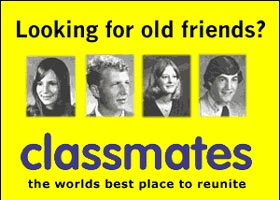
\includegraphics[width=8cm]{ressources/classmates.jpg}
    \captionof{figure}{\centering \textbf{1995: }Classmates permet de communiquer avec ses anciens camarades de classe,
    }
    \label{IMG}
    \end{center}  

\end{frame}
\begin{frame}
    \frametitle{}

    \begin{center}
    \centering
    
\includegraphics[width=8cm]{ressources/linkedin.png}
    \captionof{figure}{\centering \textbf{2002: }Linkedin est orienté sur la vie professionnelle.}
    \label{IMG}
    \end{center}

\end{frame}
\begin{frame}
    \frametitle{}

    \begin{framed}
        Peut-on catégoriser les différents réseaux sociaux?
    \end{framed}

\end{frame}
\begin{frame}
    \frametitle{}

    \begin{activite}
    \textbf{Travail oral:} 
    \begin{itemize}
        \item Citer différents réseaux sociaux.
        \item Les rassembler par catégories.
    \end{itemize}
    \end{activite}

\end{frame}
\begin{frame}
    \frametitle{}
    \begin{activite}
        Construire une carte mentale des différents réseaux sociaux, en s'inspirant du modèle ci-dessous. Choisir un réseau social par catégorie.
        \begin{center}
            \centering
            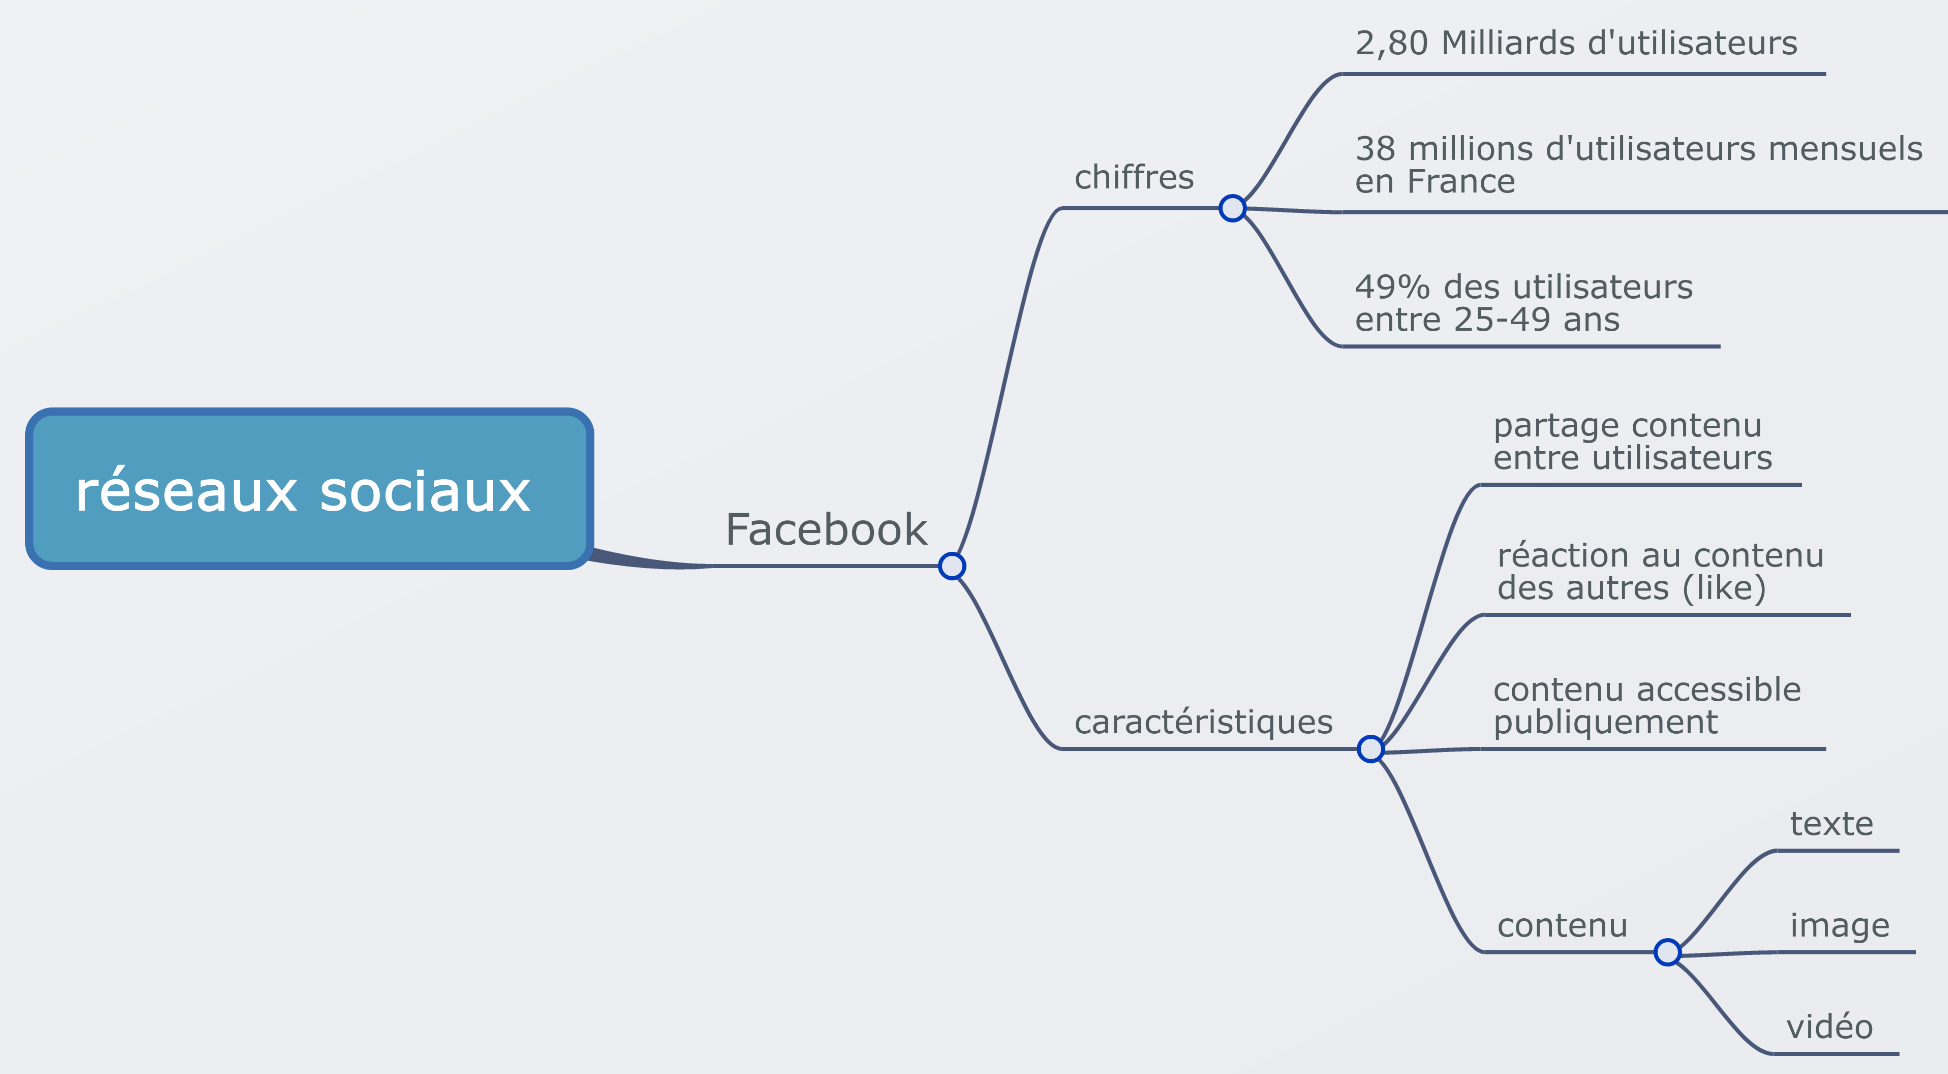
\includegraphics[width=12cm]{ressources/carte-mentale.png}
        \end{center}
        \end{activite}
    

\end{frame}
\end{document}